% Quick start guide
\documentclass{beamer}
\usetheme {Hannover}
% Title page details
\title{Garbage Collection in JVM}
\subtitle{And some tuning}
\author{Miro Kurka}
\url{https://gitlab.science.upjs.sk/mek/jvm-gc-seminar}
\institute{Pavol Jozef Safarik University}
\date{\today}
\begin{document}
\begin{frame}
% Print the title page as the first slide
\titlepage
\end{frame}
\begin{frame}{Outline}
    \tableofcontents
\end{frame}
\section{Motivation}

\section{Introduction to Garbage Collection}
\subsection{Memory Overview - Stack and Heap}
\subsection{The Idea of Garbage Collection}
\subsection{Objects in memory and How to manage them}
\subsection{Memory Allocation in Java}

\section{Garbage Collection Algorithms in JVM}
    \subsection{Serial garbage collector}
    \subsection{The throughput collector}
    \subsection{CMS}
    \subsection{G1 GC}
    
\section{Tuning - When to choose what}
    \subsection{CMS vs G1 GC}
    \subsubsection{Demo 1 - Docker app}
    \subsubsection{Demo 2 - Low latency server}


\section*{References}

\begin{frame}
    \frametitle{Motivation}
    \begin{itemize}
        \item This seminar is about \texttt{automata} and ML 
        \item Our University basic courses are in Java 
        \item Jobs in KE are usually Java
        \item Interest in low latency programming
        \item Read a paper during undergrad (they lied)
    \end{itemize}
\end{frame}
\begin{frame}

    \frametitle{Introduction to Garbage Collection}
    \begin{columns}
        \column{0.6\textwidth}
        \begin{itemize}
            \item Programs use memory
            \item You have to manage your memory (\texttt{C,C++})
            \begin{itemize}
                \item Reference counting 
                \item 70\% of bugs\footnote{https://www.chromium.org/Home/chromium-security/memory-safety/}
            \end{itemize}
            \item 1957 John McCarthy LISP
            \item All statements now are limited to OpenJDK8 - OpenJDK11
          \end{itemize}
        
        
        \column{0.4\textwidth}
        \begin{figure}
            \centering
            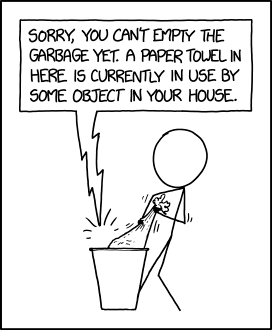
\includegraphics[width=\textwidth]{still_in_use.png}
            \caption[xkcd_1888]{Still in use\footnote{https://xkcd.com/1888/}} % Replace with your image file
        \end{figure}
        
      \end{columns}

\end{frame}
\begin{frame}
    \frametitle{Memory Overview - Stack and Heap}
    \begin{columns}
        \column{0.4\textwidth}
        \begin{itemize}
            \item JIT compiler bytecode
            \item Stack: each thread MCF\footnote{Method Call Frame}, local variables 
            \item Method Area\footnote{excluded from GC}: Metaspace or PermGen (method bytecode, metadata, static variables)
            \item \underline{Heap:} dynamically allocated objects
        \end{itemize} 
        \column{0.6\textwidth}
       
        \begin{figure}
            \centering
            \includegraphics[width=\textwidth]{images/jvmmem.png}
            \caption{Actual layout of JVM\cite{noauthor_memory_nodate}}
        \end{figure}
        
      \end{columns}
 
\end{frame}

\begin{frame}
    \frametitle{The Idea of Garbage Collection}
    \begin{columns}
        \column{0.6\textwidth}
        \begin{itemize}
            \item Objects are used often or not
            \item Hence split them into two groups!  
        \end{itemize}
        \begin{figure}
            \caption[bigdecimal]{A code snippet}
        \end{figure}
        \column{0.5\textwidth}
        \begin{figure}
            \includegraphics[width=2.9cm]{cpp_developer.png}
            \caption[dev]{A \texttt{C++} developer reminiscing about GC}
        \end{figure}

    \end{columns}
\end{frame}


\begin{frame}
    \frametitle{Serial garbage collector}
    \framesubtitle{The first}
    \begin{itemize}
        \item This was default GC algorithm implemented for JVM on 32 bit one threaded CPU's 
        \item Two steps: minor GC and full GC
        \item Stops all app threads 
    \end{itemize}
    \begin{figure}
        \includegraphics[width=\textwidth]{images/basic.png}
        \caption[javaheap]{An idealized heap\cite{book} }
    \end{figure}
\end{frame}

\begin{frame}
    \frametitle{Throughput garbage collector}
    \framesubtitle{our good friend for 64 bits}
    \begin{itemize}
        \item default until JDK7u11
        \item Again two steps: minor GC and full GC 
        \item It uses multiple threads to collect the YG
    \end{itemize}
    \begin{figure}
        \includegraphics[width = \textwidth]{images/TGC_yc.png}
        \caption[tgc_yc]{Young generation collection in Throughput algorithm}
    \end{figure}
\end{frame}

\begin{frame}
    \frametitle{Throughput garbage collector}
    \framesubtitle{The second step - Old collection}
    \begin{itemize}
        \item The old collection frees everything out of the YG (including survivor spaces)
        \item The only compactified objects that remain, are those which have active references
    \end{itemize}
    \begin{figure}
        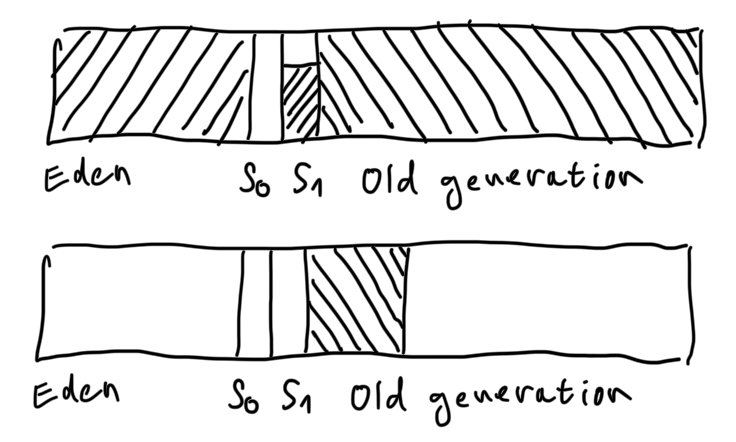
\includegraphics[width = \textwidth]{images/TGC_og.png}
        \caption[tgc_og]{Old generation collection in Throughput algorithm}
    \end{figure}
\end{frame}

\begin{frame}
    \frametitle{Tuning the Throughput GC}
    \framesubtitle{All about that balance\dots}
    \begin{itemize}
        \item Heap size vs. YC/OC gens.
        \item \texttt{-XX:MaxGCPauseMillis=N } (no default)
        \item \texttt{-XX:GCTimeRatio=N} (default = 99)
        \item (95 $\rightarrow$ 1.95\%)
        \item TGC will try to balance things out
    \end{itemize}
    \begin{equation*}

        % TODO remove numbering 
        
         $TGoal = 1 - \frac{1}{1+GCTimeRatio}$
    \end{equation*}
\end{frame}

\begin{frame}
    \frametitle{CMS - concurrent mark sweep}
    \framesubtitle{Overview and the first step }
    \begin{itemize}
        \item Works in three states
        \begin{itemize}
            \item CMS collects the YC (stops app threads)
        \end{itemize}
    \end{itemize}
    \begin{figure}
        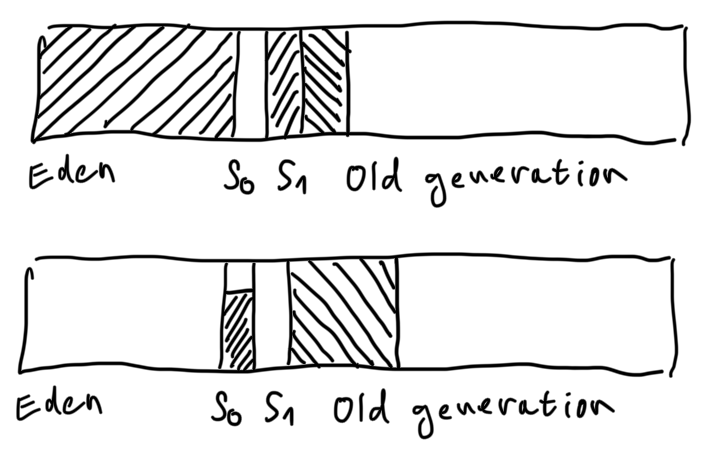
\includegraphics[width=\textwidth]{images/CMS_yg.png}
        \caption{Objects are  moved from Eden into one survivor space and into the old generation.}
    \end{figure}
\end{frame}

\begin{frame}
    \frametitle{CMS - concurrent mark sweep}
    \framesubtitle{The second step} 
    \begin{itemize}
        \item If the heap is sufficiently full JVM launches background threads
        \item Concurrently running threads clean up the old generation
        \item There is no compaction of the OG 
    \end{itemize}
    \begin{figure}
        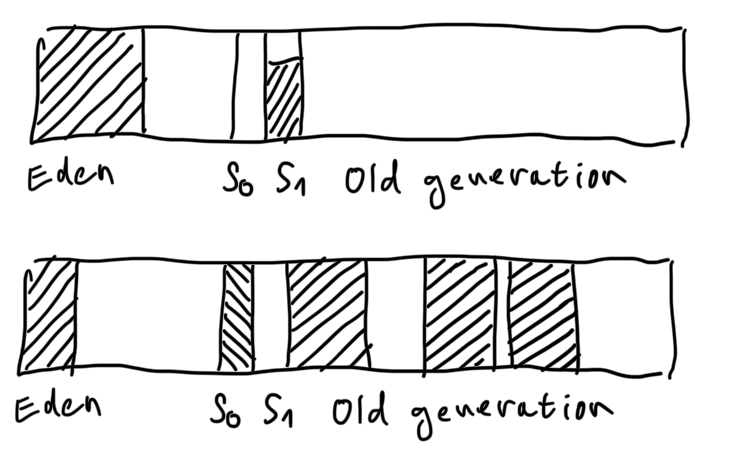
\includegraphics[width = \textwidth]{images/CMS_con.png}
        \caption{A CMS sweep}
    \end{figure}
\end{frame}
\begin{frame}
    \frametitle{CMS - concurrent mark sweep}
    \framesubtitle{What if things go wrong?} 
    \begin{itemize}
        \item Concurrent mode failure
        \begin{itemize}
            \item What? Background thread doesnt finish scanning and freeing objects in the heap before it fills up
            \item \underline{Result:} CMS has to revert to doing a full GC with all application threads stopped
            \item Solution: On the next slide
        \end{itemize}
        \item Promotion failure
        \begin{itemize}
            \item When? Old generation runs out of space before enough memory can be reclaimed from the old generation.
            \item  \underline{Result:} The heap is too fragmented, long pauses for full GC 
            \item Solution: Use G1 GC algorithm
        \end{itemize}
    \end{itemize}
\end{frame}

\begin{frame}
    \frametitle{Tuning the CMS}
    \begin{itemize}
        \item Concurrent mode failure is expensive for CMS
        \item \texttt{-XX:CMSInitiatingOccupancyFraction=N}
        \item \texttt{-XX:+UseCMSInitiatingOccupancyOnly}
        \item tells CMS at which \% of OG occupancy should background thread start
    \end{itemize}
\end{frame}

\begin{frame}
    \frametitle{G1 GC}
    \framesubtitle{An overview of the garbage first garbage collector}
    \begin{itemize}
        \item default GC since Java 11\cite{noauthor_jdk11usrchotspotsharegcg1_nodate}
        \item 4 main states 
        \begin{itemize}
            \item A young collection
            \item A concurrent cycle (in the background)
            \item A mixed collection
            \item A full GC cycle (only if necessary)
        \end{itemize}
        \item Heap has different structure, divided into many segments
        \begin{itemize}
            \item Eden (E), Survivor space (S), Old generation (O)
        \end{itemize}
    \end{itemize}
    
\end{frame}

\begin{frame}
    \frametitle{G1 GC}
    \framesubtitle{A young collection}
    \begin{figure}
        \includegraphics[width = 7cm]{images/young_collection.png}
    
    \end{figure}
    \begin{itemize}
        \item Now the outcome
    \end{itemize}
    \begin{figure}
        \includegraphics[width = 7cm]{images/outcome.png}
    
    \end{figure}
    
        
    
\end{frame}




\begin{frame}
    \frametitle{G1 GC}
    \framesubtitle{A concurrent cycle}
    
    \begin{itemize}
        \item Marking works concurrently
        \item freed Eden is being allocated 
        \item increase in size of young collection
        \item region marked with X - mostly unused objects
    \end{itemize}
    \begin{figure}
        \includegraphics[width = 7cm]{images/marking_collection.png}
    \end{figure}
\end{frame}
\begin{frame}
    \frametitle{G1 GC}
    \framesubtitle{So begins the concurrent cycle\dots}
    \begin{itemize}
        \item Here we see first phase - initial-mark phase
        \item It stops the other Java threads  
    \end{itemize}
    \begin{figure}
        \includegraphics[width = 7cm]{images/initial_mark.png}
    \end{figure}
    \begin{itemize}
        \item Root scan phase, it has to be fast (background threads avaliable) 
        
    \end{itemize}

    \begin{figure}
        \includegraphics[width = 7cm]{images/rootscan1.png}
    \end{figure}
    \begin{itemize}
        \item What can it slow down? $\rightarrow$ Objects in YC
        \item The YC is filled up quickly and has to wait for root scan
        \item Such behavior creates "longer than usual" pause
    \end{itemize}
    \begin{figure}
        \includegraphics[width = 7cm]{images/rootscan2.png}
    \end{figure}
\end{frame}

\begin{frame}

    \frametitle{G1 GC}
    \framesubtitle{A concurrent garbage collection}
    \begin{itemize}
        \item Now we are in the \texttt{concurrent} phase
        \item YC is removed with the marked X collection 
    \end{itemize}
    \begin{figure}
        \includegraphics[width = 7cm]{images/mixed_gc.png}
    \end{figure}
\end{frame}

\begin{frame}
    \frametitle{G1 GC}
    \framesubtitle{When a full GC occurs}
    \begin{itemize}
        \item G1 GC should do the least amount of full gc cycles to be effective 
        \item When they occur we can tune the Java process
        \item Usual culprits are 
        \begin{itemize}
            \item Concurrent mode failure - OG fills up $\rightarrow$ increase heap size
            \item Promotion failure - 
            \item Evacuation failure - objects from YC cant fit in the S and OG is full
            \item Humongous allocation failure - big objects allocated, causes random full GC, hard to diagnose
        \end{itemize}
    \end{itemize}

\end{frame}
\begin{frame}
    \frametitle{Tools}
    \framesubtitle{When you have a hammer everything looks like\dots}
    \begin{itemize}
        \item jcmd - command line 
        \item jconsole - live monitoring of JVM 
        \item jmap - heap dumps 
        \item jinfo - JVM properties
        \item IBM GCMV\footnote{https://www.ibm.com/support/pages/garbage-collection-and-memory-visualizer}
    \end{itemize}
\end{frame}

\begin{frame}
    \frametitle{Some of the many JVM options}
    \framesubtitle{Capture the flag!}
    \begin{itemize}
        \item GC log 
        \begin{itemize}
            \item \texttt{-XX:+PrintGC} 
            \item \texttt{-XX:+PrintGCDetails}
            \item \texttt{-Xloggc:filename}
            \item other flags for rotating, verbosity \dots
        \end{itemize}
    \end{itemize}
\end{frame}


\begin{frame}
    \frametitle{When to choose what}
    \framesubtitle{Throughput vs G1 GC}
    \begin{itemize}
        \item Lower CPU Allocation
        \item Hyper-threaded apps (Docker)
    \end{itemize}
\end{frame}


\begin{frame}
    \frametitle{Demo 1}
    \framesubtitle{One of the most used java application}
\end{frame}

\begin{frame}
    \frametitle{Demo 2}
    
\end{frame}
\begin{frame}
    \frametitle{References}
   
\end{frame}

\end{document}
